\chapter{Proposed Work and Planning}
\label{chapter:PWP}

The proposed work for the dissertation consists in the development of an
automatic compiler of DNN description into Deep Versat / IOB-RV32 C++ code. The
purpose of this work is to be able to run any state of the art CNN on the Deep
Versat system with no effort on the user side, allowing the design and
architectural exploration.

For the proof of concept stage, Darknet and Caffe will be the frameworks chosen
to be supported by the compiler. Deep Versat can customized with the number of
layers, numbers of each FU type and other options. Hence, the compiler must be
able to take the configurations into account when producing computational
datapaths for Deep Versat.

\section{Flowchart}

\begin{figure}[!htbp]
    %\centering
    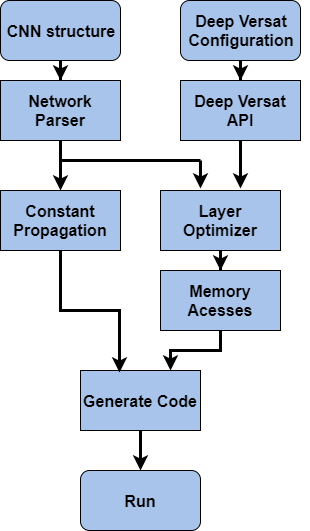
\includegraphics[width=1\textwidth]{Figures/flowchart.png}
    \caption{Flowchart of the software architecture}
    \label{figure:flowchart}
\end{figure}



Figure~\ref{figure:flowchart} presents the flowchart of the system to be developed. The mais steps
of the algorithm are explained in the next paragraphs.

%FIX Aproveitas o que está em bx para alguma box fo do fluxo grama ?
To build a CNN model for Versat, a parser from Configuration file to layer is needed. For darknet~\cite{darknet}, the parser can be re-used.
For Caffe, a new one would need to be built so the output of the parser is equal to other frameworks for the same CNN network.
The objective to be accomplished is to support all Caffe possible layers and Darknet's layers.
After parsing, the Versat dataflow and runs for each type of layer will be defined depending on current silicon set up of the CGRA. Then,
the C code with the Versat runs will be written. In~\ref{figure:cgraopt}, a CGRA optimization flow for CNN is presented.

%FIX Aproveitas para alguma box fo do fluxograma ?
Some of the activation functions discussed in chapter \ref{chapter:cnn}
will have to be processed in software on the core unless custom Functional Units
are made for each function. Convolutional,Fully Connected,Shortcut and Route
layers can be implemented on Deep Versat without any FU changes. How much it
will be accelerated is based on number of cores and MACs available. Pooling
needs adaptation in Hardware to run them, if not implemented, run on the RISC-V
core.

\section{Workplan}

In fig~\ref{figure:gant}, a GANT chart with the proposed schedule for the
planned work is presented. Further explanations on each task will follow in the
next paragraphs.

\begin{figure}[!htbp]
    %\centering
    \includegraphics[width=1\textwidth]{Figures/gant2.png}
    \caption{GANT chart of Proposed Work}
    \label{figure:gant}
\end{figure}





